% Chapter 4

\chapter{Segmentación del iris} % Main chapter title

\label{Capítulo 4} % For referencing the chapter elsewhere, use \ref{Chapter4} 

%----------------------------------------------------------------------------------------

% Define some commands to keep the formatting separated from the content 
%\newcommand{\keyword}[1]{\textbf{#1}}
%\newcommand{\tabhead}[1]{\textbf{#1}}
%\newcommand{\code}[1]{\texttt{#1}}
%\newcommand{\file}[1]{\texttt{\bfseries#1}}
%\newcommand{\option}[1]{\texttt{\itshape#1}}

%----------------------------------------------------------------------------------------

\section{Introducción}

El proceso de localizar y aislar el iris en una imagen es conocido como localización o segmentación del iris. Esta etapa juega un papel muy importante en los sistemas de reconocimiento de iris ya que la extracción de características se realiza sobre esta región obtenida, lo que provoca que una mala segmentación haga perder información discriminante sobre el iris haciendo que los SRI (sistemas de reconocimiento de iris) empeoren en sus resultados. \\

La etapa de segmentación del iris se basa en una secuencia de tareas: encontrar un iris en la imagen, determinar sus contornos interno y externo entre la pupila y la esclerótica respectivamente, detección de los bordes de los párpados superior e inferior si estos ocluyen el iris y por último detectar y excluir cualquier elemento superpuesto de pestañas o reflexiones de la córnea o de gafas. Aunque son muchos métodos para la segmentación del iris los que se han propuesto, todavía no pueden considerarse concluyentes para usarse en distintas condiciones como: condiciones de iluminación, reflexiones especulares, oclusiones por párpados, oclusiones por pestañas, entre otros. En esta tesitura existe el problema de mejorar la precisión de las segmentaciones bajo condiciones no ideales. \\

Los métodos de segmentación del iris se pueden agrupar en dos categorías: métodos basados en la detección de bordes circulares y métodos basados en la detección de bordes no circulares. En esta primera categoría se asume que el iris tiene una forma circular o elíptica en función de la perspectiva, y que se aproximan los bordes del iris utilizando dos circunferencias que en la mayoría de los casos se consideran concéntricas. En la segunda categoría los métodos se basan en la detección de bordes no circulares, asumiendo que el iris tiene una forma menos circular debido a las afecciones producidas por los factores de calidad como: oclusión por los párpados, oclusión por las pestañas, emborronado, iluminación no uniforme, reflexiones especulares, etc, provocando que la segmentación del iris sea más dificil de realizar. \\

Son varios los métodos existentes para la segmentación del iris basada en la detección de bordes circulares, siendo el método propuesto por Daugman el cual se basa en el operador integro-diferencial el más utilizado. En este sentido son varios los métodos existentes que se basan en el operador integro-diferencial para realizar la segmentación del iris. Otra bvs variantes de métodos que se han empleado para la segmentación del iris se basan en diferentes enfoques como: la detección de bordes de Canny junto con las transformada de Hough, la detección de puntos del borde del iris utilizando un modelo de atracción-repulsión basado en la ley de Hooke, la aplicación iterativa de una propuesta basada en la transformada de Hough adaptada con ponderaciones, entre otros. \\

Del mismo modo existen diversas propuestas para el método de segmentación del iris basados en la detección de bordes no circulares, donde la detección de los bordes tiene que ser lo más precisa posible ya que en este ámbito partimos en que el iris no mantiene una forma circular en condiciones no ideales debido a las afectaciones producidas por los diferentes factores de calidad como las oclusiones por pestañas o párpados que producen un efecto de distorsión sobre el mismo. Para este tipo de métodos Daugman propone una solución basada en la segmentación de los bordes internos y externos en términos de contornos activos basados en expansiones de series discretas de Fourier sobre datos de contornos. Otra implementación para este tipo de métodos es la que se propone mediante un esquema de segmentación del iris basado en la relación de contornos activos y la computación de curvas de longitud mínima llamadas "geodesics". \\



%----------------------------------------------------------------------------------------

\section{Descripción del método empleado}

Desde una vista frontal del iris se pueden apreciar dos bordes bien definidos. El primero, formado entre la pupila y el iris, está definido por el paso de los valores de menor intensidad (que representan la región de la pupila) a valores de intensidad media referidas a la región del iris. El segundo borde,comprendido entre el iris y la esclerótica está definido por el paso de los valores de intensidades medianas correspondientes a la región del iris a valores de intensidades mas altas que caracterizan la región de la esclerótica. \\

Partiendo de estas premisas y analizando los diferentes métodos de segmentación del iris mencionados en el apartado anterior, este Trabajo Fin de Master se basa en el método expuesto en \cite{Reference9}. Este método realiza primeramente una aproximación inicial del centro del iris para posteriormente segmentar los bordes interno y externo del mismo. \\

Para realizar la aproximación del centro del iris, el método parte de la suposición de que su centro es muy cercano al centro de la imagen, por lo que trata de buscar el objeto mas grande y oscuro que aparece en la imagen el cual representa la pupila (que también define el borde interno del iris). En general, el método realiza un procedimiento iterativo de análisis de perfiles desde el centro de la imagen P($X_{I}$, $Y_{I}$). Dichas operaciones de perfiles son realizadas en las direcciones horizontal ($H_{p}$) y vertical ($V_{p}$). La región donde se encuentran los puntos candidatos a centro del iris que van a ser procesados se define por la región cuadrada de tamaño 2mX2m con centro en P($X_{I}$, $Y_{I}$). Las valores de los pixeles obtenidos de las operaciones de perfiles aplicadas viene representados como segmentos de líneas rectas. Por tanto, el centro del iris representado por el punto P($X_{0}$, $Y_{0}$) es aquel en el cual $H_{p}$ y $V_{p}$ tienen los mismos valores de píxeles consecutivos que son menores que un umbral \textit{h}. En la invetigación realizada para este método se determinó que para la base de datos de iris utilizada (CASIA-IrisV4-Internal) los valores mas adecuados para los parámetros utilizados son \textit{m} = 70 y \textit{h} = 50. \\

\begin{figure}[htbp]
\centering
\subfigure{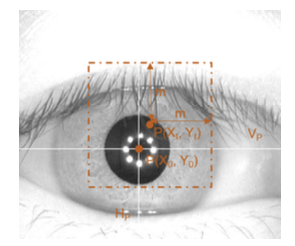
\includegraphics[width=60mm]{tfm-img53}}
\caption{Notaciones mostradas sobre un ejemplo de la base de datos CASIA-IrisV4-Internal del método empleado para la aproximación del centro del iris.} \label{fig:señales}
\end{figure}

Una vez encontrado el centro del iris en la imagen, el siguiente paso es segmentar los bordes interno y externo del mismo. Antes de realizar el proceso de segmentación de los bordes se va a aplicar un filtro mediana con el objetivo de resaltar los bordes y degradar detalles del iris. De esta manera también se eliminan las afectaciones producidas en la imagen por las reflexiones especulares y las oclusiones por pestañas. En la siguiente imagen se puede observar el resultado de la aplicación de filtrado. \\

\begin{figure}[htbp]
\centering
\subfigure[]{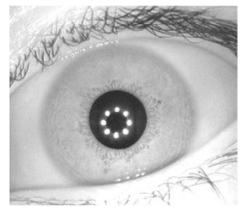
\includegraphics[width=44mm]{tfm-img54}}
\subfigure[]{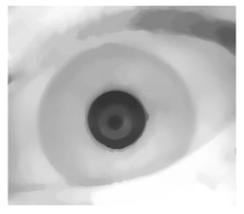
\includegraphics[width=44mm]{tfm-img55}}
\caption{Resultado de la aplicación del filtrado. (a) Imagen original. (b) Imagen con el filtrado de mediana aplicado.} \label{fig:señales}
\end{figure}

Para realizar la segmentación de los bordes interno y externo del iris, el método ejecuta dos procedimientos de búsqueda de bordes circulares sobre la imagen suavizada de la anterior figura (ver Figura 4.2). Básicamente el método trata de determinar el radio $r^{*}_{s} \epsilon R, R = \left \{ \left. r_{min}, r_{min}+1,..., r_{max}-1, r_{max} \right \} \right.$ con centro en P($X_{0}$, $Y_{0}$) haciendo uso del gradiente en las coordenadas (x,y) que es definido como el siguiente vector columna:\\

\[
\nabla f = \begin{bmatrix}
Gx\\ 
Gy
\end{bmatrix} = \begin{bmatrix}
\frac{\partial f}{\partial x}\\ 
\frac{\partial f}{\partial y}
\end{bmatrix}
\]
\captionof{figure}{Vector gradiente.}

El vector gradiente indica la dirección de mayor cambio de los valores de las intensidades de la imagen. El módulo de dicho vector, es decir, la magnitud del vector gradiente, representa la mayor tasa de crecimiento de la intensidad por unidad de distancia. \\

\[
M(x,y) = mag(\nabla f) = \sqrt{Gx^{2} + Gy^{2}}
\]
\[
M(x,y) \approx \left | Gx \right | + \left | Gy \right |
\]
\captionof{figure}{Magintud del vector gradiente.}

\[
\alpha(x,y) = tan^{-1} \left ( \frac{Gx}{Gy} \right )
\]
\captionof{figure}{Dirección del vector gradiente.} 

\begin{table}[htbp]
\begin{center}
\end{center}
\end{table}

De esta manera, se aplican arcos consecutivos en los sentidos  de s $\epsilon$ S, S $ = \left \{ \left. izquieda, derecha, arriba, abajo \right \} \right.$ dando como resultado el conjunto de puntos de interés $C_{s}(r, X_{0}, Y_{0})$ pertenecientes a dichos arcos. \\

\begin{figure}[htbp]
\centering
\subfigure[]{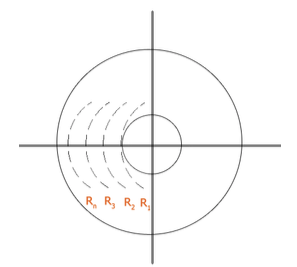
\includegraphics[width=50mm]{tfm-img56}}
\subfigure[]{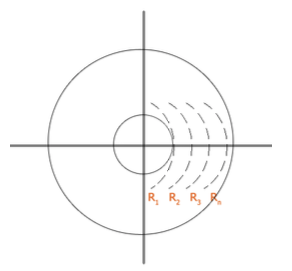
\includegraphics[width=50mm]{tfm-img57}}
\subfigure[]{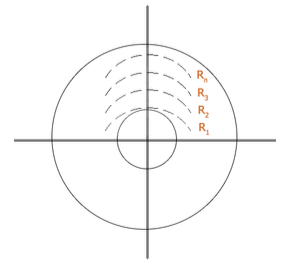
\includegraphics[width=50mm]{tfm-img58}}
\subfigure[]{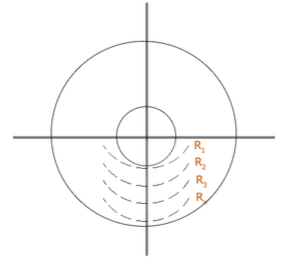
\includegraphics[width=50mm]{tfm-img59}}
\caption{Sentidos en los que se analizan los arcos sucesivos. (a) Izquieda. (b) Derecha. (c) Arriba. (d) Abajo} \label{fig:señales}
\end{figure}

\begin{figure}[htbp]
\centering
\subfigure{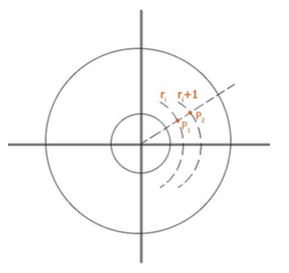
\includegraphics[width=50mm]{tfm-img60}}
\caption{Puntos de interés en dos arcos sucesivos} \label{fig:señales}
\end{figure}

En la Figura 4.6 se describe de forma gráfica los incrementos de radios para el análisis de los arcos sucesivos en el sentido \textit{S}. Del mismo modo, en la Figura 4.7 se visualiza un ejemplo de puntos de interés en dos arcos sucesivos en el sentido hacia la derecha. \\

%Tendiendo en cuenta las características del iris mencionadas anteriormente y tomando como referencia los modelos de métodos de segmentación del iris mencionados anteriormente, en este trabajo se propone un nuevo método de segmentación basado en la detección de bordes circulares compuesto por la combinación del método de Sobel para la detección de bordes y la transformada de Hough para la detección de figuras geométricas, en este caso las circunferencias que representan los bordes internos y externos del iris.\\

%Los bordes de una imagen digital se pueden definir como transiciones significativas de niveles de gris entre dos regiones. Este cambio en el valor de las intensidades de los pixeles aportan una importante información sobre las fronteras de los objetos, la cual se puede aprovechar para ser utilizada en la segmentación de la imagen, el reconocimiento de objetos, etc. El ruido también genera bordes o contornos, por lo que es importante tratar de eliminarlo antes de realizar el proceso de segmentación. La mayoría de las técnicas para detectar bordes emplean operadores locales basados en distintas aproximaciones discretas de la primera y segunda derivada de los niveles de grises de la imagen. \\

%La derivada de una señal continua proporciona las variaciones locales con respecto a la variable, en este caso nos dará los cambios que se produce en las intensidades de niveles de gris de los pixeles, de manera que el valor de la derivada es mayor cuanto más rápidas son estas variaciones siendo cero cuando dichas variaciones de intensidad entre los pixles se mantiene constante. En el caso de las funciones bidimensionales, la derivada es un vector que apunta en la dirección de la máxima variación de f(x,y) y cuyo módulo representa la cantidad de variación por unidad de distancia, lo que se conoce como gradiente. Estas derivadas son calculadas mediante operadores de convolución. \\


%\[
%\nabla f = \begin{bmatrix}
%Gx\\ 
%Gy
%\end{bmatrix} = \begin{bmatrix}
%\frac{\partial f}{\partial x}\\ 
%\frac{\partial f}{\partial y}
%\end{bmatrix}
%\]
%\captionof{figure}{Vector gradiente.}

%\[
%M(x,y) = mag(\nabla f) = \sqrt{Gx^{2} + Gy^{2}}
%\]
%\[
%M(x,y) \approx \left | Gx \right | + \left | Gy \right |
%\]
%\captionof{figure}{Magintud del vector gradiente.}

%\[
%\alpha(x,y) = tan^{-1} \left ( \frac{Gx}{Gy} \right )
%\]
%\captionof{figure}{Dirección del vector gradiente.} 

\begin{table}[htbp]
\begin{center}
\end{center}
\end{table}

%El método de Sobel queda encuadrado dentro de los operadores de primera derivada. Este método calcula el gradiente de una imagen en base a las variaciones de las intensidades de los pixeles para la detección de bordes. Este operador aplica dos filtros de convolución gaussianos, uno horizontal para la derivada en X y otro vertical para la derivada en Y con el objetivo de suavizar el ruido para que no se sobredetecten los bordes y poder calcular de manera fiable el gradiente, el cual nos dirá si un punto (pixel) de la imagen pertenece a un borde. Las máscaras de convolución de Sobel tienen un tamaño de 3x3 tanto en horizontal como en vertical, y se aplicarán al vecindario de pixeles formado alrededor del punto sobre el que se este aplicando. Este operador presenta la ventaja de ser mas sensible al ruido frente a otros operadores de primera devirvada como Roberts o Prewitt entre otros.\\ \\ \\

%\begin{table}[htbp]
%\begin{center}
%\begin{tabular}{|l|l|l|}
%\hline
%-1 & -2 & -1 \\ \hline
%0 & 0 & 0\\ \hline
%1 & 2 & 1 \\ \hline
%\end{tabular}
%\caption{Kernel gradiente filas 3x3(Gx).}
%\label{tabla:sencilla}
%\end{center}
%\end{table}

%\begin{table}[htbp]
%\begin{center}
%\begin{tabular}{|l|l|l|}
%\hline
%-1 & 0 & 1 \\ \hline
%-2 & 0 & 2 \\ \hline
%-1 & 0 & 1 \\ \hline
%\end{tabular}
%\caption{Kernel gradiente columnas 3x3 (Gy).}
%\label{tabla:sencilla}
%\end{center}
%\end{table}		

%Es importante ajustar bien el umbral de medida para la detección de bordes ya que un tamaño de umbral pequeño puede dar lugar a que se detecten falsos bordes en la imagen. Del mismo modo, un ajuste de umbral elevado puede producir que se obvien bordes que delimiten correctamene objetos en la imagen. Debido a esto se han realizado diversas experimentaciones con diferente valor de umbral para ver cual de ellos es menos discriminante de bordes y minimiza la detección de falsos positivos.\\

%\begin{figure}[htbp]
%\centering
%\subfigure[128]{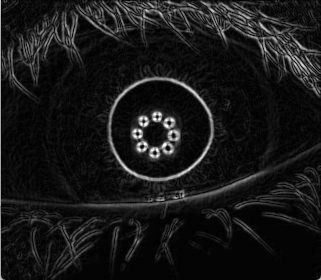
\includegraphics[width=44mm]{tfm-img28}}
%\subfigure[90]{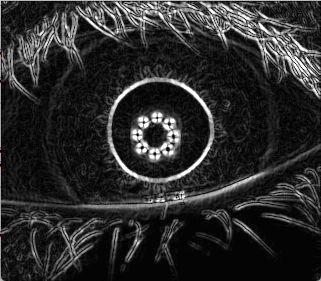
\includegraphics[width=44mm]{tfm-img29}}
%\subfigure[70]{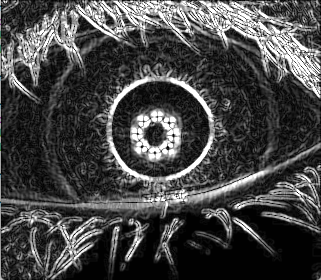
\includegraphics[width=44mm]{tfm-img30}}
%\caption{Detección de bordes sobre la imagen S1001L02.jpg de la base de datos CASIA-IrisV4-Internal con diferentes valores de umbral.} \label{fig:señales}
%\end{figure}

%Como se puede apreciar en las imagenes resultantes de la batería de pruebas realizada, un valor de umbral reducido provoca que se detecten muchas líneas dando lugar a falsos bordes. Debido a eso se ha optado por establecer un valor de umbral de 128, que como se ha podido comprobar en las imágenes es el que obtiene un mejor resultado ya que entre otras ventajas evita una sobredetección.\\

%La transformada circular de Hough es el otro método que forma parte de la combinación de estos y que da como resultado el método de segmentación del iris propuesto en este trabajo. Aunque inicialmente esta técnica solo identificaba líneas rectas en una imagen, posteriormente se extendió para detectar cualquier figura que se pudiera describir con unos parámetros. Este método utiliza los puntos de la imagen que pertenecen a bordes de posibles figuras para realizar un proceso de votación sobre un conjunto de figuras parametrizadas para ver si pertenecen a ellas. Para la detección de circunferencias se emplea un sistema de votación similar al utilizado para detectar rectas, donde cada punto vota por las circunferencias en las que pudiera estar, buscando posteriormente los picos en el acumulador para obtener el radio y el centro de la circunferencia, es decir, los puntos mas votados. \\

%\[
%\left ( x - c_{x} \right )^{2}+\left ( y - c_{y} \right )^{2} = r^{2}
%\]
%\captionof{figure}{Expresión matemática para definir una circunferencia.} 

\begin{table}[htbp]
\begin{center}
\end{center}
\end{table}

%donde \textit{r} es el radio de la circunferencia, y \textit{$c_{x}$}, \textit{$c_{y}$} son las coordenadas en el eje X y en el eje Y respectivamente del centro de la circunferencia.\\

%\begin{figure}[htbp]
%\centering
%\subfigure{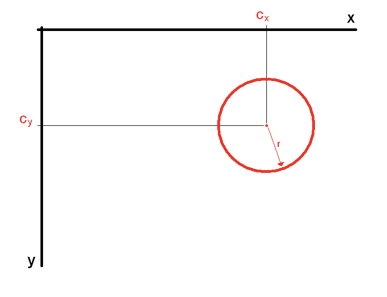
\includegraphics[width=75mm]{tfm-img31}}
%\caption{Circunferencia con centro en ($c_{x}$, $c_{y}$) y radio r.} \label{fig:señales}
%\end{figure}

%Cabe destacar que valores diferentes de ($c_{x}$, $c_{y}$ y r) proporcionan distintas circunferencias y que para cada pixel de contorno o borde de la imagen que aparece en la posición ($x_{0}$, $y_{0}$) existe una familia de circunferencias que pasan por ese punto dadas por:

%\[
%c_{x} = x_{0} + cos \theta \cdot  r
%\]
%\[
%c_{y} = y_{0} + sin \theta \cdot  r
%\]

%\begin{table}[htbp]
%\begin{center}
%\end{center}
%\end{table}

%por eso, dado unos valores de radio mínimo y máximo se calculann los valores ($c_{x}$, $c_{y}$) del centro de la circunferencia para ese radio que pasa por cada punto desde $\theta$ = 0 a $\theta$ = 360. Una vez realizados los cálculos si aparece los parámetros (las coordenadas $c_{x}$, $c_{y}$ y el radio r) de un punto en el espacio que tenga muchos votos quiere decir que corresponden a la circunferencia que pasa por una gran cantidad de puntos de contorno. \\ 

%\begin{center}
%\begin{minipage}{0.5\textwidth}
%\begin{algorithmic}
%\For {r = r\_min:r\_max}
	%\For {tetha = 0:360}
    	%\State{$c_{x}$ = $x_{0}$ + cos($\theta$) * r;}
    	%\State{$c_{y}$ = $y_{0}$ + cos($\theta$) * r;}
    	%\State{hough($c_{x}$,$c_{y}$,r) = hough($c_{x}$,$c_{y}$,r) + 1;}
	%\EndFor
%\EndFor
%\end{algorithmic}
%\end{minipage}
%\end{center}

\begin{table}[htbp]
\begin{center}
\end{center}
\end{table}

\begin{table}[htbp]
\begin{center}
\end{center}
\end{table}
%----------------------------------------------------------------------------------------

\section{Experimentaciones}

Para probar la fiablidad y robustez del método de segmentación del iris empleado, se ha decidido realizar una batería de pruebas para contrastar los resultados con los obtenidos de aplicar otros dos métodos de segmentación del iris proporcionados por la librería USIT como son Caht y Wahet, los cuales se describieron en el capítulo anterior. Las experimentaciones fueron ejecutadas en C++ utilizando un ordenador portátil Intel Core i5 a 2 GHz con 8GB de memoria RAM. Se ha utilizado la base de datos de imágenes CASIA-IrisV4-Interval, la cual contiene un total de 54.601 imágenes de iris de más de 1.800 sujetos, todas ellas tomadas bajo iluminación infrarroja cercana o sintetizada que se representan en ficheros JPEG de escala de grises de 8 bits para realizar la segmetación del iris. La elección de esta base de datos frente al otro contenedor de imágenes utilizado durante la investigación de este Trabajo Fin de Master se debe a la gran cantidad y variedad de oclusiones por párpados y pestañas que presenta CASIA-IrisV4-Interval frente a UBIRIS y que permite realizar la segmentación en unas condiciones no ideales como el método propone. Además, se estableció experimentalmente $r_{mín}$ = 20, $r_{max}$ = 70 para detectar el borde interno y $r_{mín}$ = 80, $r_{max}$ = 130 para detectar el borde externo en las imágenes de la base de datos CASIA-IrisV4-Interval, partiendo de los valores asignados anteriormente a los parámetros \textit{m} y \textit{b} . \\  \\  \\ \\ \\ \\ \\ \\ \\ \\ \\ \\ 

\begin{figure}[htbp]
\centering
\subfigure[S1001R04.jpg]{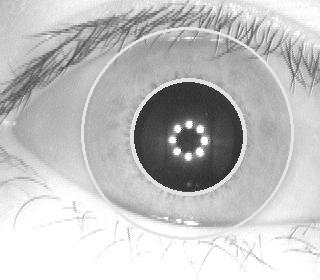
\includegraphics[width=44mm]{tfm-img36}}
\subfigure[S1115L09.jpg]{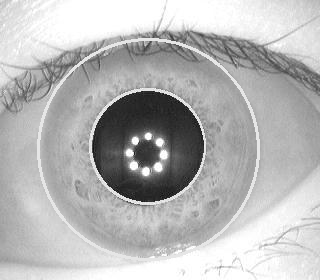
\includegraphics[width=44mm]{tfm-img37}}
\subfigure[S1136L07.jpg]{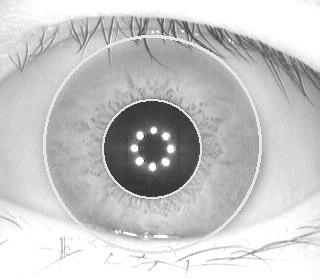
\includegraphics[width=44mm]{tfm-img38}}
\subfigure[S1143R07.jpg]{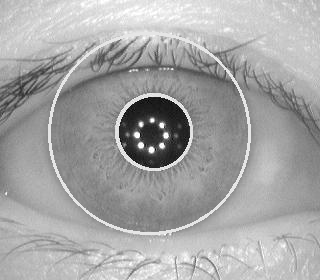
\includegraphics[width=44mm]{tfm-img39}}
\subfigure[S1208L07.jpg]{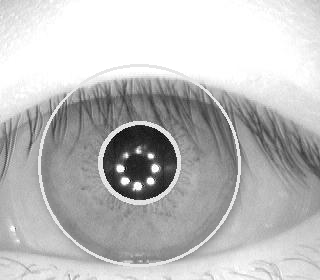
\includegraphics[width=44mm]{tfm-img46}}
\subfigure[S1209R04.jpg]{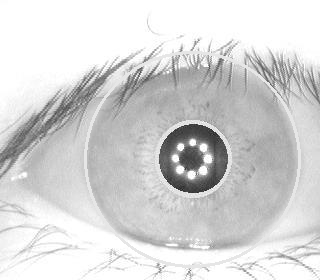
\includegraphics[width=44mm]{tfm-img47}}
\caption{Detección de los bordes del iris con el método empleado.} \label{fig:señales}
\end{figure}

\begin{figure}[htbp]
\centering
\subfigure[S1001R04.jpg]{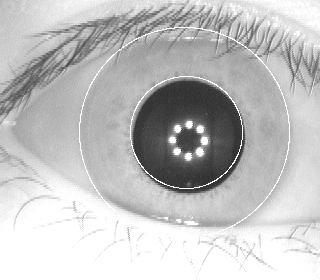
\includegraphics[width=44mm]{tfm-img32}}
\subfigure[S1115L09.jpg]{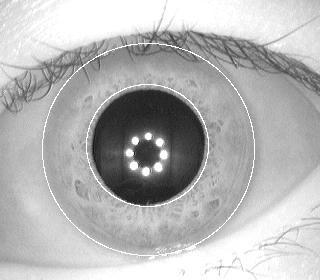
\includegraphics[width=44mm]{tfm-img33}}
\subfigure[S1136L07.jpg]{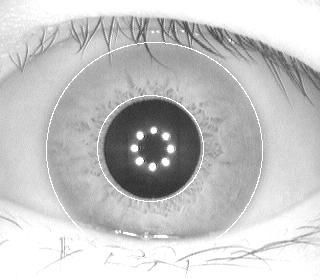
\includegraphics[width=44mm]{tfm-img34}}
\subfigure[S1143R07.jpg]{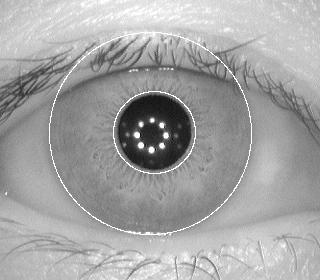
\includegraphics[width=44mm]{tfm-img35}}
\subfigure[S1208L07.jpg]{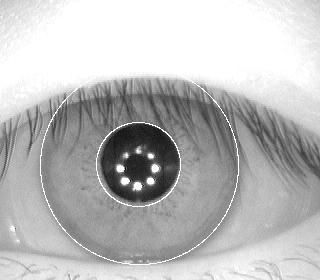
\includegraphics[width=44mm]{tfm-img44}}
\subfigure[S1209R04.jpg]{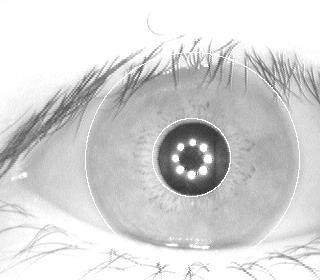
\includegraphics[width=44mm]{tfm-img45}}
\caption{Detección de los bordes del iris con el método Caht .} \label{fig:señales}
\end{figure}

\begin{figure}[htbp]
\centering
\subfigure[S1001R04.jpg]{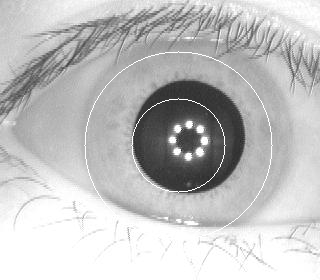
\includegraphics[width=44mm]{tfm-img40}}
\subfigure[S1115L09.jpg]{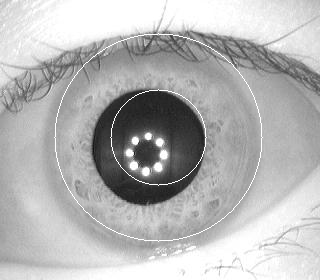
\includegraphics[width=44mm]{tfm-img41}}
\subfigure[S1136L07.jpg]{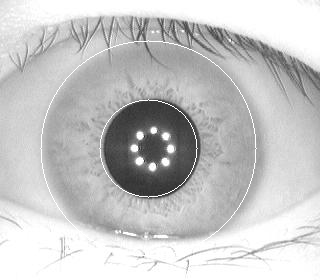
\includegraphics[width=44mm]{tfm-img42}}
\subfigure[S1143R07.jpg]{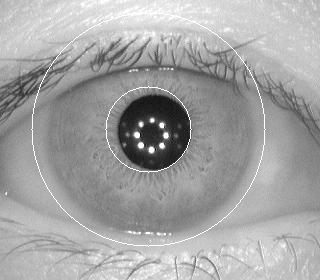
\includegraphics[width=44mm]{tfm-img43}}
\subfigure[S1208L07.jpg]{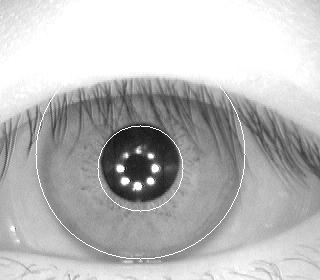
\includegraphics[width=44mm]{tfm-img48}}
\subfigure[S1209R04.jpg]{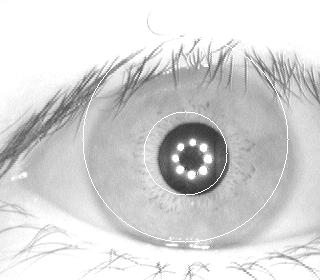
\includegraphics[width=44mm]{tfm-img49}}
\caption{Detección de los bordes del iris con el método Wahet.} \label{fig:señales}
\end{figure}


\begin{figure}[htbp]
\centering
\subfigure[S1001R04.jpg]{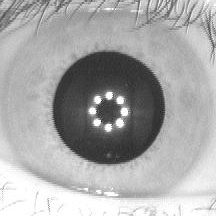
\includegraphics[width=44mm]{tfm-img61}}
\subfigure[S1115L09.jpg]{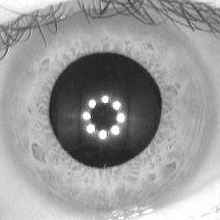
\includegraphics[width=44mm]{tfm-img62}}
\subfigure[S1136L07.jpg]{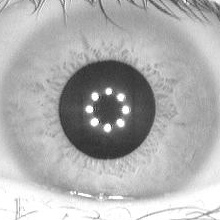
\includegraphics[width=44mm]{tfm-img63}}
\subfigure[S1143R07.jpg]{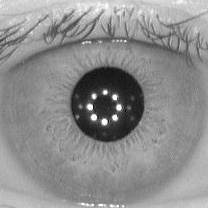
\includegraphics[width=44mm]{tfm-img64}}
\subfigure[S1208L07.jpg]{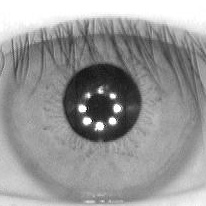
\includegraphics[width=44mm]{tfm-img65}}
\subfigure[S1209R04.jpg]{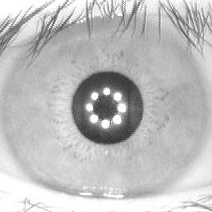
\includegraphics[width=44mm]{tfm-img66}}
\caption{Segmentación del iris con el método empleado.} \label{fig:señales}
\end{figure}

Para evaluar la calidad de los resultados que se han obtenido y que se muestran en las anteriores imágenes, se va a medir el grado de solapamiento que existe entre una segmentación de referencia y la segmentación de cada uno de los métodos mencionados anteriormente. Para la segmentación de referencia se tomará la segmentación manual realizada por un experto sobre cada una de las imágenes de la base de datos CASIA-IrisV4-Interval y para la cual se necesitó de varias sesiones debido a la gran cantidad de imágenes que esta contiene. El grado de solapamiento entre dos segmentaciones se medirá por el porcentaje de pixeles que coincidan entre las dos áreas segmentadas, siendo el 100\% el mayor grado de precisión del segmentado como se muestra en la Figura 4.12. \\ \\ \\

\begin{figure}[htbp]
\centering
\subfigure{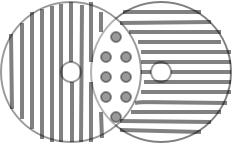
\includegraphics[width=75mm]{tfm-img50}}
\caption{Representación gráfica del solapamiento entre la segmentación de referencia y la segmentación a través de los métodos expuestos.} \label{fig:señales}
\end{figure}

\begin{table}[h]
\begin{center}
\begin{tabular}{@{}lcc@{}}
\toprule
Método empleado		& Base de datos de imágenes 		& Porcentaje calidad \\ \hline
Actual 			& CASIA-IrisV4-Interval		& 96.5\% \\
Caht 			& CASIA-IrisV4-Interval		& 91.7\% \\
Wahet  		& CASIA-IrisV4-Interval		& 79.3\% \\
\end{tabular}
\end{center}
\caption{Porcentaje de solapamiento entre la segmentación de referencia}
\label{my_tabla}
\end{table}

\begin{table}[htbp]
\begin{center}
\end{center}
\end{table}
%----------------------------------------------------------------------------------------

\section{Conclusiones}

En este Capítulo 4 se ha presentado el método de segmentación del iris que se va a emplear para la extracción de dicha región. Como se ha podido comprobar, dicho método se basa en una aproximación inicial del centro de iris a través de un proceso iterativo de análisis de perfiles (horizontal y vertical), seguido del cálculo de los radios de los bordes interno y externo del mismo a través del análisis de arcos sucesivos en los sentidos de S $ = \left \{ \left. izquieda, derecha, arriba, abajo \right \} \right.$. Para comprobar la robustez y precisión del método de segmentación del iris empleado, se ha realizado una batería de experimentaciones junto con otros métodos de la misma índole para evaluar la calidad de los resultados arrojados por estos, donde hemos podido ver como el método empleado en este trabajo fin de master es el que mejor rendimiento ha obtenido ya que ha alcanzado el porcentaje de calidad más alto que el resto de los métodos presentes. Para las pruebas realizada se establecieron unos valores de parámetros de los radios con  $r_{mín}$ = 20, $r_{max}$ = 70 para la detección del borde interno y $r_{mín}$ = 80, $r_{max}$ = 130 para la detección del borde externo, además de un valor de umbral \textit{b} = 50.\\
%En este Capítulo 4 se ha presentado un nuevo método de segmentación del iris basado en la detección de bordes circulares. El presente método está compuesto por la técnica de detección de bordes de Sobel junto con la transformada circular de Hough. A través del operador de primera derivada Sobel se consigue detectar los pixeles de la imagen que forman parte del borde o contorno de una figura predeterminada, en este caso de circunferencias. A cada uno de esos pixeles se les aplica la transformada circular de Hough para detectar las circunferencias que conforman el límite interno y límite externo del iris, calculando los valores $c_{x}$ y $c_{y}$ para las múltiples y diversas circunferencias que pasan por cada uno de estos puntos desde $\theta$ = 0 a $\theta$ = 360 dado unos valores de radio mínimo y máximo. Los parámetros $c_{x}$, $c_{y}$ y r que más votos acumulen serán los que definan la circunferencia que representa el límite interno del iris, siendo representado el límite externo por la circunferencia formada por los segundos parámetros más votados. Se han realizado una serie de pruebas para ajustar el valor del umbral en el operador de Sobel de manera que no se produzcan muchos falsos positivos ni se discrimen bordes pertenecientes a objetos dentro de la imagen. Para comprobar la robustez y precisión del método de segmentación del iris propuesto, se ha realizado una batería de experimentaciones junto con otros métodos de la misma índole para evaluar la calidad de los resultados arrojados por estos, donde hemos podido ver como el método propuesto en este trabajo fin de master es el que mejor rendimiento ha obtenido ya que ha alcanzado el porcentaje de calidad más alto que el resto de los métodos presentes.\\ 

%----------------------------------------------------------------------------------------